\chapter{Practical approach to software metrics} \label{roz:metrics-practic}

\textit{The purpose of this chapter is to use software metrics to improve the quality of code for exemplary academic project. Basing on tools introduced in Chapter~\ref{roz:metrics-tools} (STAN, RefactorIT and JHawk) and metrics described in Chapter~\ref{roz:metrics_theory}, the project is analysed and it is underlined which aspects need improvements.}

\section{Project description}
The research made in this chapter are based on academic project of implementing neural network and algorithms that uses neural network to compute the results of its exploratory areas. The Figure~\ref{fig:structureneural} presents coupling between the package. The structure has been generated with use of STAN plug-in for Eclipse \ac{IDE}. 

\begin{figure}[h!]
 	\centering
 	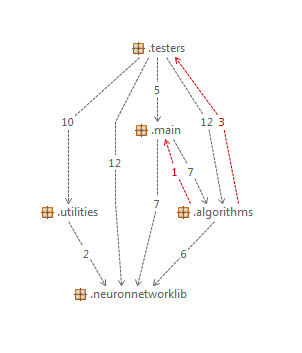
\includegraphics[scale=1]{img/str.png} 
 	\caption{Neural network project structure}		
 	\label{fig:structureneural}
 \end{figure} 

\section{Metrics analysis}
The Figure~\ref{fig:wyniki} presents the results of measurement with use of size metrics, object-oriented metric (\ac{CK metrics}) and package metric (Martin's metrics) for neural network project.  

\begin{figure}[h!]
	\centering
	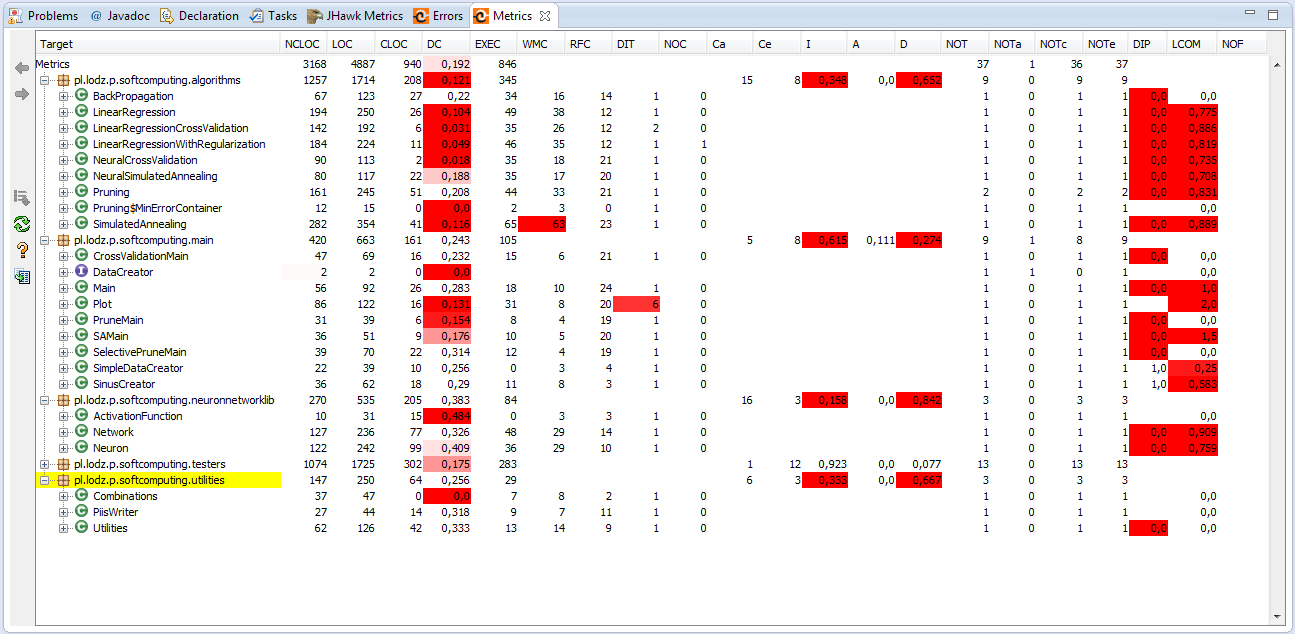
\includegraphics[scale=0.45]{img/wyniki-refactorIT.png} 
	\caption{The results for neural network project generated by RefactorIT.}		
	\label{fig:wyniki}
\end{figure}

\subsubsection*{Size metrics}
The Lines of Code (\ac{LoC}) metric in RefactorIT does not take into account comments, empty lines and imports. The non-commented lines of code (\ac{NCLOC}) counts the lines that are not comments or empty lines. The commented lines of code (\ac{CLOC}) informs how many lines contains comments or Java docs. The executable statements (\ac{EXEC} indicates the lines that are executable statements. 

The main function of already mentioned metrics and these from NOT--family metrics (number of types (\ac{NOT}), number of abstract types (\ac{NOTa}), number of concrete types (\ac{NOTc}), number of exported types (\ac{NOTe})) is to inform about the size of project. The greater values are, the more effort has been taken to prepare the implementation. In this case, any values exceeding is predicted. 

The density of comments (\ac{DC}) metric determines a density value of how commented the code is. The red background indicated that there are classes which are not enough commented. In other words, there are no Java docs provided for every class, method or attribute in given package.

\subsubsection*{Object-oriented metrics}
The next group studied by RefactorIT tool is \ac{CK metrics}. According to NASA publication \cite{nasa} that made the research about object-oriented projects. In complex system, 60\% of class have \ac{WMC} values smaller than 20, about 36\% between 20 and 100, and only 4\% of class have \ac{WMC} greater than 100. In this case, the neural network project has only one class (\texttt{SimulatedAnnealing}) that exceeds desired value. It means that it is the most complex class and it needs to be reimplemented. The difference in compare to rest of classes is really high. 

The greater \ac{RFC} value is, the more complex and functional class is. It causes problems in testing and maintenance. Analysing \ac{RFC} values for neutral network project, it could be stated that the most complex are classes which values exceed 20. They are usually in \textit{pl.lodz.p.softcomputing.algorithms} package what proves the definition of \ac{RFC}.       

In case of \ac{DIT} metric, the greater number of class that given child class inherits, the deeper degree of complexity is. It increases the cost of maintenance, so the class chain that leads to \texttt{Plot} class should be shorten. 

The next from \ac{CK metrics} set is \ac{LCOM} metric, but more precisely LCOM2 metric. The results should be returned in interval between 0 and 1. The smallest values are the better. As it could be observed, the area of improvements in that case is very wide. It indicates lack of cohesion inside the methods.  

The results of \ac{NOC} metric shows that inheritance is poorly used in neural network project which could lead to code duplication. The \ac{CBO} metric is not implemented in RefactorIT.

\subsubsection*{Martin's metric}
The Martin's metrics that into consideration the packages inside the neural network project. The upper limit for values of efferent coupling (\ac{Ce}) is 20. Neither of packages exceed it. The same situation is with afferent coupling (\ac{Ca}), however the tolerance for \ac{Ca} is equal even to 500. 

The abstractness (\ac{A}) calculates the relationship between number of interfaces and classes within the package. Only for a one package this ratio has been calculated (\textit{pl.lodz.p.soft\-com\-pu\-ting.main}). The resultant value means that the package is open to changes in implementation.

The instability (\ac{I}) calculated the effort needed to change a package without impacting others. The stability of the package is defined in range 0.0 to 0.3. In this case of \textit{pl.lodz.p.soft\-com\-pu\-ting.al\-go\-rithms, pl.lodz.p.soft\-com\-pu\-ting.neu\-ron\-net\-work\-lib} and \textit{pl.\-lodz.\-p.\-soft\-com\-pu\-ting.u\-ti\-li\-ties} packages could be stated that are or are closed to be treated as stable. The packages: \textit{pl.lodz.p.soft\-com\-pu\-ting.main} and \textit{pl.lodz.p.soft\-com\-pu\-ting.tes\-ters} are considered as unstable or as close to be unstable packages.

The last from Martin's metrics set is distance from the main square (\ac{D}). The values close to 0 are desirable ones. Any package that is not close to zero is considered as unbalanced and need to be reimplemented to be less sensitive to changes~\cite{martin}. The only acceptable is value for \textit{pl.lodz.p.soft\-com\-pu\-ting.tes\-ters} package. The values for the rest of packages are not acceptable. 

\subsubsection*{Halstead complexity metrics}
The Halstead complexity metrics are implemented only in JHawk plug-in. The shareware version of JHawk enables to calculate four of metrics: program length, program volume difficulty error proneness and effort to implement but only on package or class level. It is not possible to generates those results for the whole project in freeware version. The Figure~\ref{fig:jhawk3} presents the results for  \textit{pl.lodz.p.soft\-com\-pu\-ting.al\-go\-rithms} package. 

\begin{figure}[h!]
	\centering
	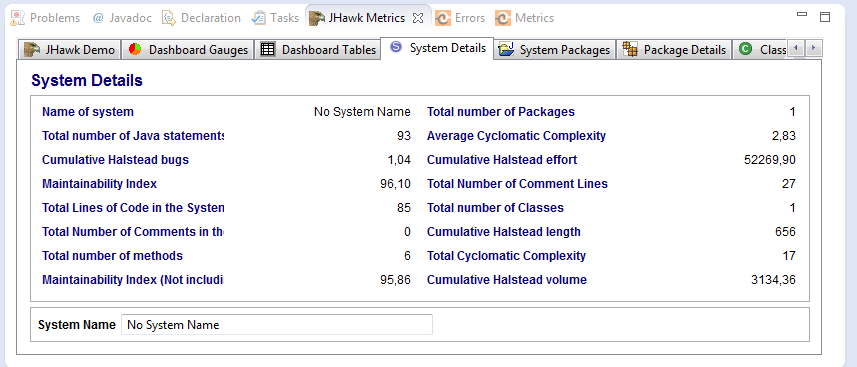
\includegraphics[scale=0.7]{img/jhawk3.png}  
	\caption{Results of Halstead metrics generated by JHawk plug-in.}		
	\label{fig:jhawk3}
\end{figure}

The results of program level and time to implement metrics could be very easily derived from provided formulas described in section~\ref{sec:halstead}. 

For program level (L):
\[L=\frac { 1 }{ 1,04 } \approx 0,96\]

For time to implement (T):
\[T=\frac { 52699,9 }{ 18 } \approx 2903,88\quad seconds\]

Basing on the results could be stated that implementation of researched package requires \textit{48~minutes and 24~seconds}. The obtained result is only theoretical and does not take into consideration any external factors.  

\subsubsection*{McCabe's cyclomatic complexity}

Using STAN plug-in, it is possible to calculate average cyclomatic complexity of overall project and for each of the package:
\begin{verbatim}
Average cyclomatic complexity of overall project = 2.59
pl.lodz.p.softcomputing.algorithms = 2.89
pl.lodz.p.softcomputing.neuronnetworklib = 1.79 
pl.lodz.p.softcomputing.utilities = 3,64
pl.lodz.p.softcomputing.main = 1.9
pl.lodz.p.softcomputing.testers = 2.72
\end{verbatim}

The complexity should be analysed on method levels, however the ratio on package level shows which package contains the most complex classes and methods.

\section{Summary}
Basing on the results provided by the metric tools it could be concluded that the inheritance mechanism in project is poorly developed. Using inheritance enables to prevent duplicated of code. Another aspect is a fact that the code is not enough documented. It is a very good practise to provide documentation with the system for further development in the future. 

The lack of cohesion and not satisfactory result of Martin's metrics indicates that package division and information exchange between methods and classes need to be redesigned and improved. 

The results of the Halstead metric should be treated with caution, because they have not use at design level and are based on very changeable aspects.

Even if the recommended value of some metric is exceeded it does not mean that it is necessary to refactor the code. The metrics violations are rather a warning about an increased risk of faults appearance and potential problems with further maintenance. 

Th resultant values should be considered as a reference point because depending on the specific system recommended values are varied. Because of that fact, many tools enables to modify  recommended values. 
